\documentclass[a4paper]{scrartcl}%{{{

\usepackage{float}
\usepackage{tikz}
\usetikzlibrary{arrows,automata}
\usepackage{pgf}
\usepackage[utf8]{inputenc} % this is needed for umlauts
\usepackage[ngerman]{babel} % this is needed for umlauts
\usepackage[T1]{fontenc}    % this is needed for correct output of umlauts in pd
\usepackage{amssymb}
\usepackage{amsmath}
\usepackage{mathabx}
\usepackage{mathrsfs}
\usepackage{dsfont}
\usepackage{graphicx}
\usepackage{fancyhdr}
\usepackage{lastpage}
\usepackage{imakeidx}
\setlength{\parskip}{\medskipamount}
\setlength{\parindent}{0pt}
\usepackage{enumitem}
\usepackage{hyperref}
\usepackage{verbatim}

%%%%%%%%%%%%%%%%%%%%%%%%
% Kopf- und Fusszeilen %
%%%%%%%%%%%%%%%%%%%%%%%%
\pagestyle{fancy}
\lhead{
        Maximilian Roth
}
\chead{Logik-Tutorat Lösungen Blatt 9\\}
\rhead{
    \begin{tabular}{rr}
        \today{} \\
        Seite \thepage{} von \pageref{LastPage}
    \end{tabular}
}
\lfoot{}
\cfoot{}
\rfoot{} 

%%%%%%%%%%%%%%%%%%%%%%%%
% Anfang des Dokuments %
%%%%%%%%%%%%%%%%%%%%%%%%%}}}

\begin{document}
\section*{Disclaimer}%{{{
\label{sec:disclaimer}
Auch in diesem Dokument können sich Fehler befinden!\\
Sie sind nicht die Musterlösung der Aufgaben, sondern selbst erstellte Lösungen.\\

Als generelle Lektüre kann ich nur das Skript von Markus Junker aus dem WS 17/18 empfehlen:\\
\url{http://home.mathematik.uni-freiburg.de/junker/skripte/InfoLogik.pdf}\\
Hier ist vieles sehr genau und verständlich erklärt.%}}}

\section*{}%{{{
\label{sec:aufgabe_1}

    \begin{figure}[H]
        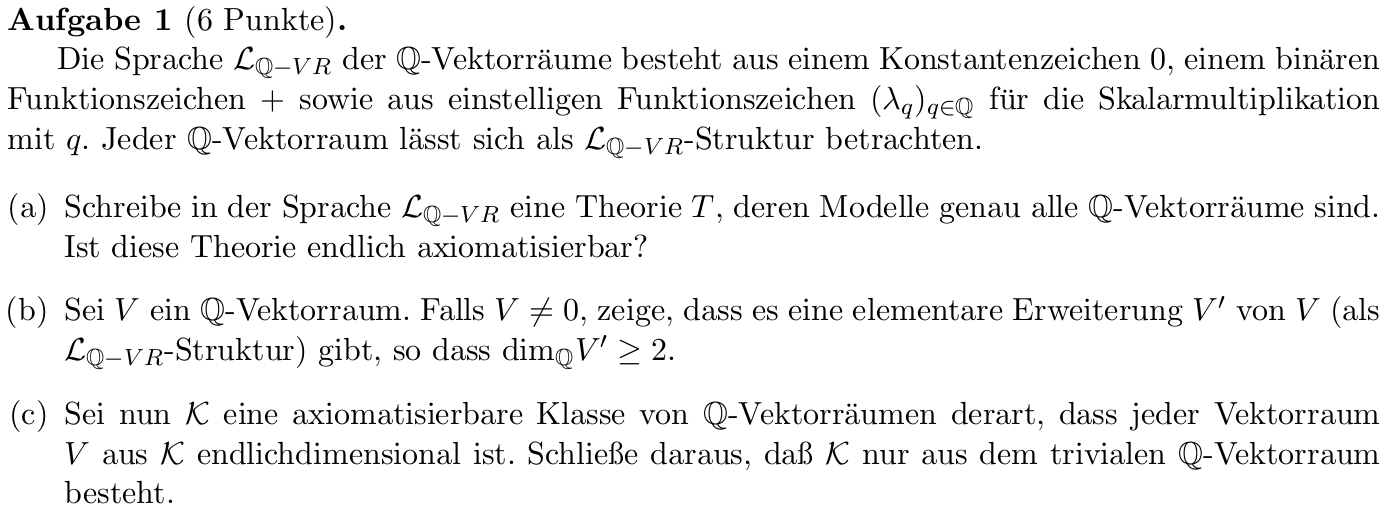
\includegraphics[scale=0.3]{./A-1.png}
        \label{fig:}
    \end{figure}

    \begin{itemize}
        \item a)\\
            Für $a,b \in \mathds{Q}$\\
            $T =\\
            \{\forall u \forall v \forall w (u + (v + w)) \doteq ((u + v) + w)\} \cup\\
            \{\forall v \forall w ((v + w) \doteq (w + v))\} \cup\\
            \{\forall v (v + 0) \doteq v\} \bigcup \cup\\
            \{\forall v \exists w (v + w) \doteq 0\} \cup\\
            \\$Und für alle a,b $\in \mathds{Q}\\
            \{\forall v \forall w (\lambda_a(v + w) \doteq (\lambda_a(v) + \lambda_a(w)))\} \cup\\
            \{\forall v \lambda_1(v) \doteq v\} \cup\\
            \{\forall v (\lambda_{a+b}(v) \doteq (\lambda_a(v) + \lambda_b(v)))\} \cup\\
            \{\forall v (\lambda_{a \cdot b}(v) \doteq \lambda_a(\lambda_b(v)))\}$\\
            \\Nein, da dies für alle a,b gelten muss und es damit unendlich viele Aussagen sind.\\
        \item b)\\
            Wir suchen also eine elementare Erweiterung V' in der gilt: $\exists c \exists v$: c und v sind linear unabhängig.\\ 
            \underline{Formal:} $V' \vDash Diag(V) \cup \{\neg \lambda_q(d_v) \doteq c | q \in \mathds{Q}\}$\\
            $d_v$ benötigen wir, um die Formel klar für \underline{ein}  v auszudrücken\\
            \\Also erweitern wir unsere Sprache um die $d_v, \forall v \in V\backslash \{0\}$, sowie das c.\\
            \\Jetzt nutzen wir den Kompaktheitssatz:\\
            Seien also $q_1,\dots,q_n \in \mathds{Q}$\\
            Wenn wir jetzt c wie folgt interpretieren:\\
            $c^{V'} \in V \backslash \{\lambda_{q_1},\dots,\lambda_{q_n}\}$, dann ist:\\
            $V' \vDash Diag(V) \cup \{\neg \lambda_{q_1}(d_v) \doteq c, \dots, \neg \lambda_{q_n}(d_v) \doteq c \}$ und damit konsistent.\\
            \\$\Rightarrow$ Nach Kompaktheitssatz ist damit $Diag(V) \cup \{\neg \lambda_q(d_v) \doteq c | q \in \mathds{Q}\}$ konsistent.\\
            \\Damit existiert ein V' mit den Eigenschaften.\\
        \item c)\\
            Wir nehmen an, dass $\mathcal{K}$ nicht nur aus dem trivialen Vektorraum besteht und führen dies zum Widerspruch.\\
            \\Stimmt dies, so existiert ein $\mathds{Q}-VR$ V mit $dim V \geq 1$\\
            V kann dabei jede beliebige Dimension > 0 haben.\\
            Wenn T $\mathcal{K}$ axiomatisiert, dann muss T also alle Dimensionen zulassen.\\
            \\\underline{Sprich:} Für beliebige $k_1,\dots,k_n \in \mathds{N}$ muss gelten:\\
            $T \cup $\{Es gibt $k_i$ lin. unab. Vektoren $| 1 \leq i \leq n\}\}$\\
            $\overset{Kompakth.}{\Rightarrow}$ T lässt beliebige Dimensionen zu.\\
            \\Widerspruch zu $\mathcal{K}$ endlichdimensional.\\
            $\Rightarrow \mathcal{K}$ ist nur der triviale VR.\\ 
    \end{itemize}

%}}}

\section*{}%
\label{sec:aufgabe_2}%{{{

    \begin{figure}[H]
        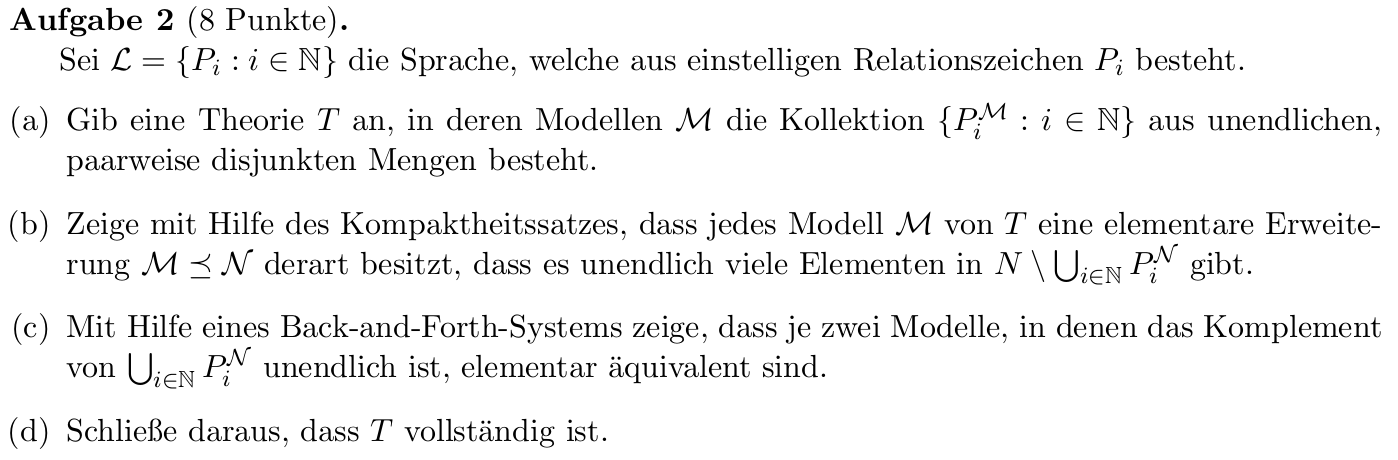
\includegraphics[scale=0.3]{./A-2.png}
        \label{fig:}
    \end{figure}

    \begin{itemize}
        \item a)\\
            Unsere Theorie muss enthalten:\\%{{{
            \begin{itemize}
                \item Jedes $P_i^\mathcal{M}$ hat unendlich viele verschiedene Elemente\\
                \item Je zwei $P_i, P_j$ haben kein gleiches Element\\
            \end{itemize}
            Und als Theorie:\\
            $T = \{\exists k_1,\dots,k_n(\bigwedge_{i \neq j} \neg k_i \doteq k_j) \land P_x(k_i)| n,x \in \mathds{N}, i,j\leq n\}\\
            \cup \{\neg \exists x (P_i(x) \land P_j(x)) | i \neq j \in \mathds{N}\}$\\%}}}

        \item b)\\
            $\mathcal{N}$ muss also unendlich viele Elemente $c_1, c_2,\dots$ haben für die gilt: $c_i \notin \bigcup_{i\in \mathds{N}}P_j^\mathcal{N}$\\
            Wir zeigen mit dem Kompaktheitssatz und erweitern dafür $ \mathscr{L} \text{ um } c_1,c_2,\dots$\\
            \\Also muss die Theorie $Diag(\mathcal{M}) \cup \{\neg c_i \doteq c_j | i\neq j \in \mathds{N}\} \cup \{\neg P_j(c_i) | j,i \in \mathds{N}\}$ konsistent sein.\\

        \item c)\\
            Wir zeigen, dass es ein nichtleeres Back \& Forth-System mit der Kollektion S gibt.\\%{{{
            
            \begin{itemize}
                \item S ist nichtleer\\
                    Seien $\mathcal{M}, \mathcal{N}$ solche Strukturen.\\
                    Wenn gilt $n \in P_i^\mathcal{N} \text{, sowie } m \in P_j^\mathcal{M}$, dann ist $F: \{n\} \rightarrow \{m\}$ partieller Iso.\\
                    Dies geht immer, da die $P_i$ existieren und unendlich groß sein müssen.\\
                    $\Rightarrow$ S ist nichtleer\\
                \item Back \& Forth-System\\
                    \begin{itemize}
                        \item \framebox{Back}\\
                            Sei $F \in S, n \in N\backslash Im(F)$\\
                            \\Wir unterscheiden in: \underline{n ist in einer Menge $P_i$} und \underline{n ist nicht in einer Menge $P_i$}\\
                            \begin{itemize}
                                \item $n \in P_i^\mathcal{N}, i \in \mathds{N}\\
                                    \Rightarrow m \in P_j^\mathcal{M} \backslash Dom(F)$\\
                                    Dabei muss m möglicherweise passend gewählt werden, wenn bereits ein $n' \in P_i^\mathcal{N}$ in Im(F) ist.\\
                                    Es ist jedoch immer möglich ein m zu finden, da alle $P_k$ unendlich groß sind und es unendlich viele davon gibt.\\
                                \item $n \notin P_i^\mathcal{N}, i \in \mathds{N}\\
                                    \Rightarrow m \in M \backslash \bigcup_{i \in \mathds{N}}P_i^\mathcal{M} \cap M \backslash Dom(F)$\\
                                    Das ist ebenfalls immer möglich, da $M, M \backslash \bigcup_{i \in \mathds{N}}P_i^\mathcal{M}$ unendlich groß sind und Dom(F) endlich groß.\\
                            \end{itemize}
                        \item \framebox{Forth} ist analog.\\
                    \end{itemize}%}}}
            \end{itemize}
    \end{itemize}
%}}}

\section*{}%{{{
\label{sec:aufgabe_3}

    \begin{figure}[H]
        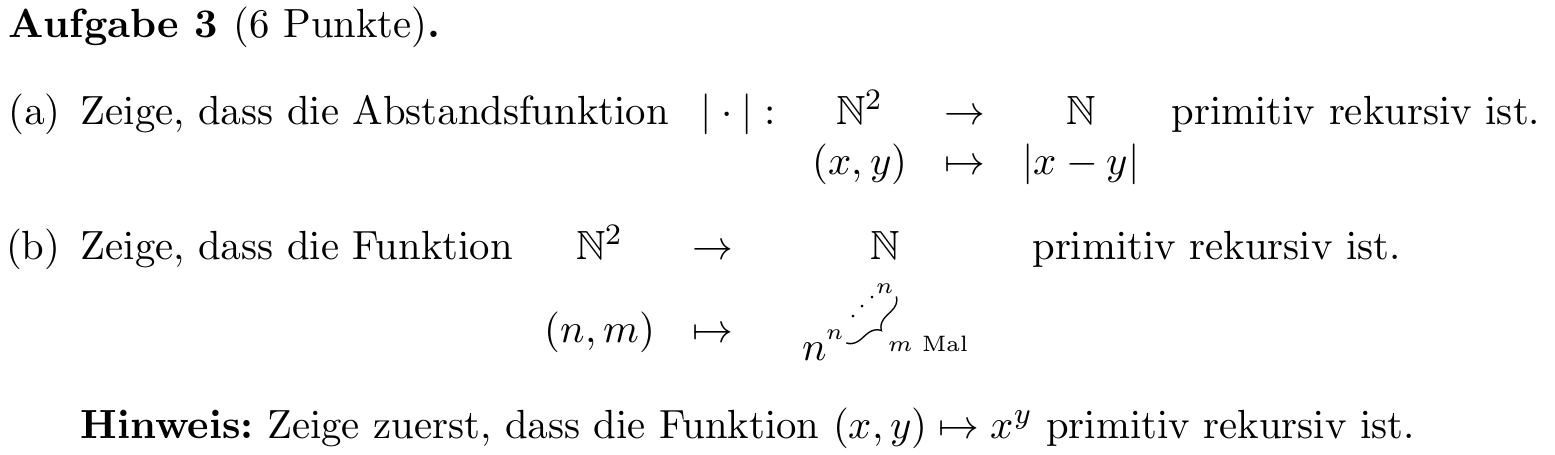
\includegraphics[scale=0.3]{./A-3.png}
        \label{fig:}
    \end{figure}

    \begin{itemize}
        \item a)\\
            $|x-y| := (x \dotdiv y) + (y \dotdiv x)$\\
            Sowohl +, als auch $\dotdiv$ sind p. rek.\\
        \item b)\\
            Wir zeigen $x^y$ p. rek.:\\
            $x^y := \begin{cases}
                        1, &\text{ falls }y=0\\
                        x \cdot x^{y-1}, &\text{ sonst }
                    \end{cases}$\\
            \\Und damit jetzt:\\
            $f(n,m) = \begin{cases}
                n, &\text{ falls }m=0\\
                n^{f(n,m-1)}, &\text{ sonst}
            \end{cases}$\\

    \end{itemize}

    
%}}}

\end{document}

